\documentclass{article}
\usepackage{amsmath}
\usepackage{graphicx}
\usepackage{tikz}
\usepackage[strings]{underscore}
\usetikzlibrary{automata,arrows,positioning,calc}

\begin{document}

\title{Monte Carlo, Markov Chains, and Monopoly}
\author{Evan Henke}

\maketitle

\begin{abstract}
\textit{Monopoly} is a classic board game that relies on randomness, in the form of rolling dice, to move players around a board.  Players will buy properties and eventually one player will win because they have gained the most money.  Using Monte Carlo simulations and Markov Chains, this paper will demonstrate that there exists a function that converges to an optimal probability that is dependent on the other players' probabilities to buy on a given side of the board.  But although this probability exists, it is not realistically calculable in a quick sitting, or player turn, and due to the nature of \textit{Monopoly's} gameplay, it is safer to play by a simple rule like that of buying 9 times out of 10.
\end{abstract}


\section{Introduction}

Over the last 70 years \textit{Monopoly} has emerged as one of the world’s most played and most well known board games.  The game pits a few friends against each other to see who can accumulate the most money.  Every player has a pawn that they move around the board and purchase the spaces or properties that they land on, the distance each pawn moves depends on the outcome of a roll of two dice.  Naturally, this causes the game to rely heavily on randomness because a player can choose if they want to purchase a property, but they cannot directly choose which property they are going to buy. Therefore, much of the game can be boiled down to to a single question of whether or not the player should purchase the properties they land on.

\subsection{History and Gameplay}

People have been playing \textit{Monopoly}, or games similar to it, for close to a century but most people are unaware that \textit{Monopoly} is a derivative of a different board game called \textit{The Landlord’s Game}.  Originally created by a woman named Elizabeth Magie, \textit{The Landlord’s Game} was made as an educational tool.  Magie was a Georgist, and the staple belief of the Georgist ideology is that economic value coming from land should be divided equally among every member of society.  Compounding on this, she held the belief that rent served only one purpose: to enrich the landlord at the expense of the tenant.  Magie wanted to teach young children this ideology so that they would grow up to be "level-headed adults" but she thought that the concept was too tough to grasp without a good example. Therefore, she decided to create a board game to demonstrate her ideals.\cite{monopolyhistory}


\begin{figure}
    \includegraphics[width=6.0in]{landlordsgame}
    \caption{Early rendition of \textit{The Landlord's Game}\cite{landlordpicture}}
    \label{landlordsgame_image}
\end{figure}


Magie had her game patented in 1904 and approached Parker Brothers to produce it.  Parker Brothers refused due to the games complexity but she was determined and she was able to have her game produced by smaller publishing companies and over time the game spread. But, with popularity comes imitation, and soon enough many others tried to replicate \textit{The Landlord’s Game} and its success.  The most notably imitation being \textit{Monopoly}, which ironically, was produced by Parker Brothers and claimed to have been created solely by a man named Charles Darrow.\cite{monopolyhistory}

Parker Brothers began production of \textit{Monopoly} in 1935, this is when it began to take the form that is widely recognized, with the iconic mascot Rich Uncle Pennybags following a year later.\cite{monopolyhistory}  The board has nine spaces on each side with one space on each corner: Go, Jail, Go to Jail, and Free Parking, for a total of 40 spaces.  Each space on the board is different. There are five properties available for player purchase on the first and four side and six on the second and third side.  Along each side of the board, there are two sets of color coded properties on each side of the board and if one player owns both or all three properties in the set, then they are said to have a monopoly at that location on the board.  There is also one utility property on each side of the board as well as three Chance spaces, three Community Chest spaces, and two Tax spaces scattered around the board.  In addition the game comes with 32 house pieces and 12 hotel pieces.\cite{rules}

Every player will begin the game with 1200 dollars and their pawn will start on Go. On their turn, the player will roll two dice and move the number of spaces indicated by the sum of their roll.  Depending on where the player lands due to their dice roll, they would have to take a certain action.  For example, Chance and Community Chest spaces make the player draw a card and take an action depending on the card text, whereas the Tax spaces requires the player to simply lose the amount of money indicated on the space on the board. However, if the player lands on a property then one of two things will happen depending on whether or not the property is owned.  If no one owns the property, whichever player landed on it has the opportunity to purchase it.  If they decide they want the property, they pay the indicated price on board and add that property to their collection. However, if they decide not to buy it then the property is put up for auction and any player that would want to purchase that property can put a bid down for it.  Whoever is willing to pay the most will purchase the property.  If the player lands on a property that is owned by another player, they must pay a sum of money to the owner of the property that depends on whether or not the owner has a monopoly at that location.  In the event that the owned location is part of a monopoly, the amount of money owed will still vary depending on whether the monopoly has houses or a hotel.  Having a monopoly means that a single player owns one the entire set of two or three properties of the same color.\cite{rules}

When a player owns a monopoly, he or she has the option to purchase houses on those properties.  Each individual property will specify how much a house will cost and the player must be able to afford to put a house on every property in that monopoly if they opt to purchase houses.  For example, if a player owns a monopoly with three properties: property A requires 100 dollars for a house, property B requires 110 dollars, and property C requires 120 dollars.  The player must be able to pay the total of 330 dollars to be able to place a house on each property in that monopoly.  The amount of money the owner gains from an opposing player landing on the space increases for every house placed on that property up to a maximum of four houses.  If a player has four houses on each property in their monopoly, he or she can choose to purchase a hotel to be placed on each property.  Hotels function very similarly to houses in that the player must be able to afford to buy enough hotels as to have one on each property and they will increase the amount the owner gains if an opposing player lands there. However, when a hotel is purchased, the four houses are removed from the property and will go back into the house pool.\cite{rules}\footnote{This differentiation is important because a popular strategy is to upgrade a player's monopoly to have four houses and but never upgrade to hotels.  The number of houses is finite, so if a player can build four houses on one monopoly they have the potential of holding twelve of the 32 houses on only one set of properties, effectively monopolizing the available houses as well as the properties they are on, but the action of purchasing a hotel will return those houses back to the available pool.\cite{strat}} 

In addition to those previously mentioned, there a few other important spaces on the board.  On each side there will be one of four utility tiles which function almost identically to that of normal monopoly properties in that a player earns more if they own more of those spaces, with the exception that these spaces cannot have houses or hotels.  Go is where players start and whenever a player lands on Go or passes Go they are given 200 dollars, unless stated otherwise by a card action.  Free Parking is a free space and nothing happens when a player ends their turn at that location.  The Go to Jail space sends the player to Jail if they end their turn there.  Jail is the final special space that needs mentioning because it is fairly important.  Jail is the second corner that a player will pass when rounding the board and it is two spaces in one: In Jail or Just Visiting.  If the player is moving by normal means onto the jail space they are said to be just visiting and nothing special happens, it is similar to Free Parking in that way. However, if the player lands on the Go to Jail space or are sent to Jail by a card action, then their pawn is moved to the Jail space and they are said to be "In Jail".  If a player is in jail they can do one of two things, roll the dice or pay 50 dollars.  Paying 50 dollars will place them into the Just Visiting part of the space and they can continue to play on their next turn.  Or the player can roll the dice and if they roll doubles then they leave jail as if they had paid the 50 dollars.  If they fail the roll then they stay in jail and can retry the roll on their next turn or pay the 50 dollars.  A player can leave jail after their third turn of being in jail.\cite{rules}
	
If a player lands and an owned property and does not have the funds to pay the owner, they can mortgage their properties.  This means they gain a small sum of money determined by the property that was mortgaged.  A mortgaged property is still owned by the same player, but the owner cannot gain income from that property. In other words, if a player lands on a mortgaged property, they are not required to pay the owner.\cite{rules}

A huge part of the game is player trading.  On a player’s turn, they can propose a trade with another player for properties or cash.  There are no true stipulations to how this trade is conducted and no player is required to accept an offer.  This gives each game of Monopoly more variety but is extremely difficult to model due to the individuality of players.

\textit{Monopoly} is not advertised as a sinister game, it is portrayed as vibrantly, fun, family game where to goal just happens to be to have the most money at the end of the game but it quickly becomes apperent that the game is more devious than the players are lead to believe. A common criticism of  \textit{Monopoly}is game's randomness as well as how the competition works.  Unlike many other competitve board games, \textit{Monopoly} relies heavily on some-what of a truce system in trading mentioned above.  Players will make these trades and deals with other players, but there can be only one winner so at some point truces are broken and this can disuade people from playing this game often, or even more than once.  So, despite the game's advertisements, many of Magie's beliefs still lives on in many peoples' distaste for the game's ruthlessness.

\section{The Simulation}

There are a number of things that complicate simulating \textit{Monopoly} that do not directly affect the game’s main function, which is to roll dice to move around the board and to purchase properties.  Therefore houses, hotels, Community Chest cards, Chance cards, property auctions, mortgaging, and trading have been removed to give a more bare-bones approach.

\subsection{Monte Carlo Methods}

There are many conditionals within the rules which can cause difficulties with the modeling approach, and this is why Monte Carlo simulations will be beneficial.  The goal is to find some optimal probability to purchase a property on the board, but this is problematic because it depends on a very large number of factors, including each individual player’s probability to buy as well as which states are available, how much money the current player has, etc.  In \textit{Monopoly}, these previously mentioned variables rely, directly or indirectly, upon the probability of being at a specific spot on the board at a certain time.  A textbook optimization problem, in most instances, could be solved using some arithmetical approximation akin to Newton's Method but in this case a distinct function, \textit{f} is not apparent, let alone finding it's derivative.

Monte Carlo simulations stress that a mathematical model can be solved using random numbers, which lends itself perfectly to this predicament.\cite{montecarlo}  Implementing the idea that the use of random numbers can lead to a non-random solution, we can begin to simulate games of Monopoly with random purchasing probabilities in the hopes to find optimal purchase strategies.

\subsection{Markov Chains, Expected Values, and Finite-State Machines}

So far this is an extremely general starting point, it has been established that there are going to be a huge number of games played, but now what?  Following the rules in playing order says that the first thing a player is going to do is to roll two dice to move their pawn around the board, so there must be a way to emulate the movements of each pawn.

A Markov Chain is a stochastic process that is composed by a set of states that follow the \textit{Markov Property}, which can also be described as being \textit{memoryless}.  In terms of a Markov Chain, this means that the future state depends only on the current state and not the \textit{history}, or previous set of states.\cite{montecarlo}

\begin{figure}
\begin{center}
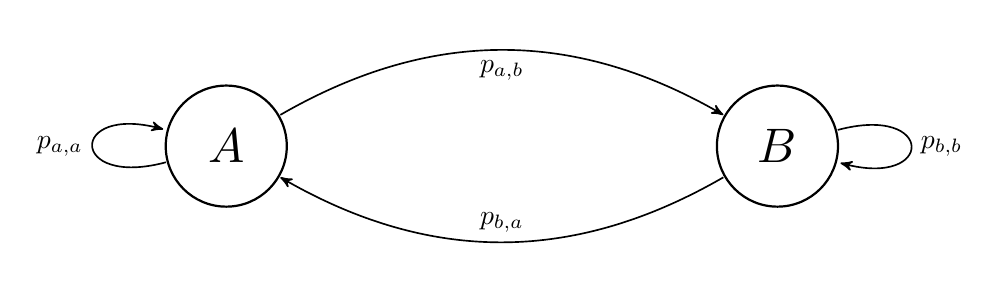
\begin{tikzpicture}[->, >=stealth', auto, semithick, node distance=4cm]
\tikzstyle{every state}=[fill=white,draw=black,thick,text=black,thick,scale=1.75]
\node[state]    (A)                     {$A$};
\node[state]    (B)[right of=A]   {$B$};
\path
(A) edge[loop left]     node{$p_{a,a}$}         (A)
    edge[bend left,below]     node{$p_{a,b}$}     (B)
(B) edge[loop right]     node{$p_{b,b}$}         (B)
    edge[bend left,above]     node{$p_{b,a}$}     (A);
\end{tikzpicture}
\caption{Example of a Markov Chain with two states A and B and their respective transition probabilities}
\label{fig:figure3}
\end{center}
\end{figure}

A Markov Chain can be envisioned as a group of points on a graph, called \textit{states} each state has \textit{transition probabilities} associated with it that will dictate the probability of transitioning from the current state to the specific state.  For example,  $p_{i,j}$ would be the probability to go from state \textit{i} to state \textit{j}.  All of these probabilities are part of a \textit{Transition Matrix}  P\cite{montecarlo} where:

$$
P=
\begin{bmatrix}
p_{0,0} & p_{0,1} & p_{0,2} & ... & p_{0,j}\\
p_{1,0} & p_{1,1} & p_{1,2} & ... & p_{1,j}\\
p_{2,0} & p_{2,1} & p_{2,2} & ... & p_{2,j}\\
... & ... & ... & ... & ...\\
p_{i,0} & p_{i,1} & p_{i,2} & ... & p_{i,j}
\end{bmatrix}
$$

So for this basic example P is a 2x2 matrix in the form

$$
P= 
\begin{bmatrix}
p_{a,a}&p_{a,b}\\
p_{b,a}&p_{b,b}
\end{bmatrix}
$$

At a high-level, a \textit{finite-state machine} is a model used for software design that, as the name implies, assumes a that the program will have a finite amount of states and that it will only be in one state at a time. \cite{finitestate} For example, if someone needed to model the motion of a door then that person could define the entire system of the door as a finite-state machine with only two states: the door is open or the door is closed.  There is some sort of function or method that will cause the finite-state machine to switch states.  In this example, when the door is in the closed state it would have a function that opens the door and the opened state would have a corresponding function to close the door.

We can think of the \textit{Monopoly} board as a finite-state machine.  The first step is to define each property on the board to be a state, giving a finite total of forty states.  A player moves between two to twelve spaces away from where they are currently positioned on the board.  Next, the transition matrix P, must be defined.  P will be in the form:

$$
P=
\begin{bmatrix}
p_{0,0} & p_{0,1} & p_{0,2} & ... & p_{0,39}\\
p_{1,0} & p_{1,1} & p_{1,2} & ... & p_{1,39}\\
p_{2,0} & p_{2,1} & p_{2,2} & ... & p_{2,39}\\
... & ... & ... & ... & ...\\
p_{39,0} & p_{39,1} & p_{39,2} & ... & p_{39,39}
\end{bmatrix}
$$

To give values for each $p_{i,j}$  the expected outcomes when two dice are rolled is considered.  The probabilities of getting a specific outcome on the dice roll can be shown in an array with the probability, $p_i$, of rolling the value of i, where i = 1,2,...,12.

$$
\setcounter{MaxMatrixCols}{20}
p=
\begin{bmatrix}
0&\frac{1}{36}&\frac{1}{18}&\frac{1}{12}&\frac{1}{9}&\frac{5}{36}&\frac{1}{6}&\frac{5}{36}&\frac{1}{9}&\frac{1}{12}&\frac{1}{18}&\frac{1}{36}\\
\end{bmatrix}
$$

These probabilities are used to create a 40x40 transition matrix for the board.  For example, if a player is on the jail space, i = 10,  then $P_i$ being the $i^{th}$ row of transition matrix P:

$$
\setcounter{MaxMatrixCols}{20}
P_i=
\begin{bmatrix}
p_0 = 0.0& ... & p_{11} = 0.0 & p_{12} = \frac{1}{36}&...& p_{22} = \frac{1}{36}& p_{23} = 0.0 & ... & p{39} = 0.0\\
\end{bmatrix}
$$

One glaring difference is on index $i = 30$, this index indicates the Go to Jail space and will always have a probability of zero.  To offset this, the Jail space will always gain that corresponding transition probability to simulate the action of moving the pawn to the jail space due to landing on Go to Jail.  

Now that movement has been covered, the rest of the simulation can be built.

\subsection{Building the Simulation}

The simulation is broken into three parts: single games, rounds, and overall averaging.  A game, as the name implies, is only one game with a single winner.  Whereas a round constitutes playing one thousand games.  Every player will have a counter that will increase with how many games they have won per round.

Each game will start with four players, simply named Player One, Player Two, Player Three, and Player Four.  Player One is the player that will be optimized around and will act slightly different than the other three players.  Each player will start on Go with 1200 dollars and an initial probability to buy that is randomly chosen between zero and one for each side of the board, with the exception that Player One will have a static initial probability to buy on each side of .50.  The players will cycle around the board using the transition matrix P, mentioned earlier.  The first and fourth sides of the board have five available properties to purchase and the second and third sides have six properties to purchase.  The simulation contains two arrays, one that tells if the property is available for purchase and the other array stores the owner of the property if it is owned.  When a player lands on a property the game will check both of these arrays for an owner, and if the property has no owner then the player will buy the property with that player’s respective probability to buy on that side of the board.  If the property is owned then the player will pay the owner an amount according to the side of the board as well as how many properties the owner has in their possession.  Each player will have a turn and if they land on a property that they cannot afford, they are removed from the game and their owned properties are returned to their unowned state and become available for purchase by the remaining players.  This will go on until one player wins.  

Once a round is complete whichever player has the most wins is deemed the round winner.  At this point the winner’s probability to win will be saved and the probabilities of Player One will be be adjusted according to the following weighted adjustment:

\begin{equation}
    \label{probability_adjustment}
    p_{i+1,n} = \alpha_i p_{i,n} + (1-\alpha_i)p_{winner,n}
\end{equation}

Where $p_i$ and $p_{i+1}$ are probabilities to buy on side $n$ ($n = 1,2,3,4$) and $\alpha_i$ is a constant that will be varied for different simulations.

This encompasses a single simulation, but in the spirit of Monte Carlo methods, there will need to be more simulations.  The simulation is run thirty times and the final value for the buying probability for each of the four sides is saved.  The average value of these final probabilities will be called the \textit{general average} for it's corresponding side of the board.

Initially players Two, Three, and Four have a buying probability between zero and one but later runs will use this average as a baseline and alter the probability to buy to see how the simulation reacts.

\section{Results and Discussion}

In this section the results of varying simulations will be shown and discussed.  The first thing that is discussed will be is the expected outcomes of the simulation.  Next $\alpha_i$ will be modified in the hopes of finding a convergent optimal probability $p_{optimal,s}$ on a given side s.  This is followed by adjustments to the probability window and various changes to how \textit{Monopoly} is played in an effort to see the reaction of $p_{optimal,s}$.

\subsection{Expectations}

To win in \textit{Monopoly} a player must purchase properties and the more properties that the player owns, the more likely it is that an opponents land on the first player's properties.  So, roughtly speaking, it is expected that the probability to buy on a side to be high.  Furthermore, due to differing property values and differing number of properties on a given side, it is also expected that the probability to buy to vary depending on the side of the board.

When Markov Chains are taught, it is not uncommon to use \textit{Monopoly} as an example, so there is no shortage of information on \textit{Monopoly}.  But what is important for us is the steady-state vector for the board.  In terms of a game of \textit{Monopoly} the steady-state vector is a collection of probabilities($s_i$ where $i = 0,1,2,....,39$) of where a player will be at a given time.  From the steady-state vector the relative frequency that a player is in Jail is by-far the largest, at .11724, the next closest is over seven percent less at .02990.\cite{dartmouth}

The \textit{expected value}, as the name suggests, is the value of a Random Variable that has the highest probability of appearing, i.e. it is what is expected to appear. \cite{montecarlo}. This value is important because the expected outcome of rolling two dice is easily calculable to be 7 and it follows that the expected outcome of rolling two dice over two turns is 14.  This means that players will be moving over sides two and three more than sides one and two.  Therefore, it is expected of those two sides to be purchased at a higher probability than that of the first and the fourth side.

\subsection{Initial Results}

Simulations will vary in two aspects:  the size of $\alpha_i$ and the \textit{probability window}, $\omega_{c,s}$, which we will define as the difference between the maximum probability and minimum probability centered about probability c on side s.  For example $\omega_{0.50,2} = .20$ would be defined as the window from $0.40$ to $0.60$ because it is of size $0.20$ centered around the value $0.50$ on the second side($\omega_{c,s} = 1$ implies that the window is the entire set of possible probabilities from zero to one).

The first step was to vary $\alpha_i$ while keeping keeping a constant $\omega_{c,s} = 1$.  Initially, we make the assumption that $\lim_{\alpha_i\rightarrow 1}\sigma_i = 0$ due to how $p_{i+1}$ was defined. The results are kept in Tables 1, 2, and 3.  

\begin{table}[h!]
\centering
\caption{Average Values for $\alpha_i = 0.9$ with $\omega_{c,s} = 1$}
\label{tab:table1}
\begin{tabular}{|c|c|c|c|}
\hline
Side & Average $p_i$ & Standard Deviation & Variance\\
\hline
1 & 0.8203074242 & 0.040839359 & 0.0016678532\\
2 & 0.8910287708 & 0.0276067073 & 0.0007621303\\
3 & 0.905966587 & 0.0204380301 & 0.0004177131\\
4 & 0.8785991185 & 0.0280977615 & 0.0007894842\\
\hline
\end{tabular}
\end{table}

\begin{table}[h!]
\centering
\caption{Average Values for $\alpha_i = 0.99$ with $\omega_{c,s} = 1$}
\label{tab:table1}
\begin{tabular}{|c|c|c|c|}
\hline
Side & Average $p_i$ & Standard Deviation & Variance\\
\hline
1 & 0.807603148 & 0.019313276 & 0.000373003\\
2 & 0.87750807 & 0.013404922 & 0.000179692\\
3 & 0.898804895 & 0.013240082 & 0.0001753\\
4 & 0.873359701 & 0.014231473 & 0.000202535\\
\hline
\end{tabular}
\end{table}

\begin{table}[h!]
\centering
\caption{Average Values for $\alpha_i = 0.999$ with $\omega_{c,s} = 1$}
\label{tab:table1}
\begin{tabular}{|c|c|c|c|}
\hline
Side & Average $p_i$ & Standard Deviation & Variance\\
\hline
1 & 0.789819981 & 0.004523793 & 2.04647E-05\\
2 & 0.863308345 & 0.002313867 & 5.35398E-06\\
3 & 0.887882061 & 0.002148036 & 4.61406E-06\\
4 & 0.861980883 & 0.002834187 & 8.03262E-06\\
\hline
\end{tabular}
\end{table}

As assumed, as $\alpha_i$ converges to 1, $\sigma_i$ shrinks.  But the big surprise is how small $\sigma_i$ is even with a full window, $\omega_{c,s} = 1$.

As $\alpha_i$ gets closer to 1, more rounds need to be ran to appear to approach a convergent solution.  On the low end 5000 rounds were ran for $\alpha_i = 0.9$ and 200,000 rounds for $\alpha_i = 0.999$.  To give a more accurate graphical representation both $\alpha_i = 0.9$ and $\alpha_i = 0.99$ were ran 200,000 times for comparison to the $\alpha_i = 0.999$ values and those are pictured in Figures 3,4,5, and 6.

\begin{figure}[htp]
\centering
\includegraphics[width=.8\textwidth]{images/ai9side1x200000}\hfill
\includegraphics[width=.8\textwidth]{images/ai99side1x200000}\hfill
\includegraphics[width=.8\textwidth]{images/ai999side1x200000}
\caption{Graph of $p_i$ on the y-axis in a single simulation over 200,000 rounds on the x-axis. From top to bottom, $\alpha_i = 0.9, 0.99, 0.999$ on side one.  Notice the decrease in variation as $\alpha_i$ gets close to 1.}
\label{fig:figure3}
\end{figure}

\begin{figure}[htp]
\centering
\includegraphics[width=.8\textwidth]{images/ai9side2x200000}\hfill
\includegraphics[width=.8\textwidth]{images/ai99side2x200000}\hfill
\includegraphics[width=.8\textwidth]{images/ai999side2x200000}
\caption{Graph of $p_i$ on the y-axis in a single simulation over 200,000 rounds on the x-axis. From top to bottom, $\alpha_i = 0.9, 0.99, 0.999$ on side two.  Notice the decrease in variation as $\alpha_i$ gets close to 1.}
\label{fig:figure3}
\end{figure}

\begin{figure}[htp]
\centering
\includegraphics[width=.8\textwidth]{images/ai9side3x200000}\hfill
\includegraphics[width=.8\textwidth]{images/ai99side3x200000}\hfill
\includegraphics[width=.8\textwidth]{images/ai999side3x200000}
\caption{Graph of $p_i$ on the y-axis in a single simulation over 200,000 rounds on the x-axis. From top to bottom, $\alpha_i = 0.9, 0.99, 0.999$ on side three.  Notice the decrease in variation as $\alpha_i$ gets close to 1.}
\label{fig:figure3}
\end{figure}

\begin{figure}[htp]
\centering
\includegraphics[width=.8\textwidth]{images/ai9side4x200000}\hfill
\includegraphics[width=.8\textwidth]{images/ai99side4x200000}\hfill
\includegraphics[width=.8\textwidth]{images/ai999side4x200000}
\caption{Graph of $p_i$ on the y-axis in a single simulation over 200,000 rounds on the x-axis. From top to bottom, $\alpha_i = 0.9, 0.99, 0.999$ on side four.  Notice the decrease in variation as $\alpha_i$ gets close to 1.}
\label{fig:figure3}
\end{figure}

\subsection{Varying the Probability Window}

With such a small deviation the thought is to reduce $\omega_{c,s}$ around the average of their respective $\alpha_i$ and side to see what happens.  For this experiment the use of only $\alpha_i = 0.99$ is sufficient because the deviation is already quite small and the amount of time to run the simulation is significantly lower than that of $\alpha_i = 0.999$.  Setting $\omega_{c,s} = 0.4$ and $\omega_{c,s} = 0.2$ as the first two windows to evaluate centered around the general average for $\alpha_i =  0.99$.  The results are in Tables 4 and 5, respectively.

\begin{table}[h!]
\centering
\caption{Average Values for $\alpha_i = 0.99$ with $\omega_{c,s} = 0.4$}
\label{tab:table1}
\begin{tabular}{|c|c|c|c|c|}
\hline
Side  & Centered Around c & Average $p_i$ & Standard Deviation & Variance\\
\hline
1 & 0.807603148 & 0.860462447 & 0.007753085 & 0.000060110334\\
2 & 0.87750807 & 0.898130494 & 0.005789447 & 0.000033517693\\
3 & 0.898804895 & 0.914810143 & 0.004411178 & 0.0000194585\\
4 & 0.873359701 & 0.8978265 & 0.004674069 & 0.0000218469199\\
\hline
\end{tabular}
\end{table}

\begin{table}[h!]
\centering
\caption{Average Values for $\alpha_i = 0.99$ with $\omega_{c,s} = 0.2$}
\label{tab:table1}
\begin{tabular}{|c|c|c|c|c|}
\hline
Side  & Centered Around c & Average $p_i$ & Standard Deviation & Variance\\
\hline
1 & 0.807603148 & 0.823715044 & 0.001086344 & 1.18014E-06\\
2 & 0.87750807 & 0.898156638 & 0.001364272 & 1.86124E-06\\
3 & 0.898804895 & 0.924639045 & 0.001033281 & 1.06767E-06\\
4 & 0.873359701 & 0.898555805 & 0.001166616 & 1.36099E-06\\
\hline
\end{tabular}
\end{table}

The first thing to notice is that the average values are not the same across different probability windows.  By using the general average as the center of the window the final result was not the same value as the general average, it was not even within a standard deviation of that value.  As a continuation of this experiment the value of $\omega_{c,s}$ will be set to be a constant that is center about a much lower value than that of the general average in such a way that the general average is not in the probility window.  If it is suspected that the optimal probability is in a close vicinity to the general average then the experimental average for this simulation would be the maximum value of the window.

\begin{table}[h!]
\centering
\caption{Average Values for $\alpha_i = 0.99$ with $\omega_{c,s} = 0.2$}
\label{tab:table1}
\begin{tabular}{|c|c|c|c|c|}
\hline
Side  & Centered Around c & Average $p_i$ & Standard Deviation & Variance\\
\hline
1 & 0.40 & 0.427064312 & 0.003882672 & 0.00001507514\\
2 & 0.45 & 0.492191439 & 0.003539403 & 0.00001252737\\
3 & 0.50 & 0.550079608 & 0.002700408 & 7.2922E-06\\
4 & 0.45 & 0.495842442 & 0.00285502 & 8.15114E-06\\
\hline
\end{tabular}
\end{table}

\begin{figure}[htp]
\centering
\includegraphics[width=.7\textwidth]{images/ai99lowprobside1}\hfill
\includegraphics[width=.7\textwidth]{images/ai99lowprobside2}\hfill
\includegraphics[width=.7\textwidth]{images/ai99lowprobside3}\hfill
\includegraphics[width=.7\textwidth]{images/ai99lowprobside4}
\caption{Graph of $p_i$ on the y-axis in a single simulation over 200,000 rounds on the x-axis of the lowered center of the probability window where $\omega_{c,s} = 0.4$, $\omega_{c,s} = 0.45$, $\omega_{c,s} = 0.50$, and $\omega_{c,s} = 0.45$ from top to bottom respectively and scaling is from 0.41 to 0.51, 0.48 to 5.05, 0.50 to 0.57, and 0.48 to 0.58 respectively.}
\label{fig:figure3}
\end{figure}

Table 6 shows the output for the lowered center and Figure 7 graphs the results.  These results imply that the optimal value is not equivalent to the general average but that it is related to the endpoints of the probability window.  More specifically, that there is a convergent value for a player's probability to buy a property that depends on the probabilities of the other players.  This can be portrayed as a function, $f$ where.

\begin{equation}
\centering
p_{optimal,s} = f(\omega_{c,s})
\end{equation}


\subsection{Relevance}

A basic function that converges to an optimal probability to purchase a property on a side is dependent on the probabilities of the other players, i.e. the probability window $\omega_{c,s}$, but what does this this mean to the player?  \textit{Monopoly} is a family game and can be an interesting modeling problem, but it is not played in a competitve fashion in the same way that games like \textit{Blackjack} or \textit{Texas Hold'em} are.  Additionally, the average player is not going to be looking for a hard and fast percentage of when they should buy because when the game is being played, it would be in a friendly manner.  

That being said, if it is assumed that the opponents are competent players, meaning they know that they must buy at a high percentage to win, then the main player should follow suit and purchase at a high probability.  A safe ratio of would be to purchase a property 8 or 9 times out of 10 assuming they can afford the property.

\subsection{Other Comments}

At the start of a game of \textit{Monopoly} every player starts with 1200 dollars and because the amount of money a player has directly affects how many properties they can purchase, any alteration to this would create a noticable change in the probabilities to buy.  Logically one would expect that if a player starts with less money then they are going to favor less expensive properties due the possibility of losing quickly if they purchase an expensive property. And vice versa, we would expect players to favor more expensive properties if they start with a larger amount.  Varying amounts for starting money are shown in Tables 7 and 8.

\begin{table}[h!]
\centering
\caption{Starting Money = 500}
\label{tab:table1}
\begin{tabular}{|c|c|c|c|}
\hline
Side  & Average $p_i$ & Standard Deviation & Variance\\
\hline
1 &  0.813392354 & 0.007994897 & 6.39184E-05\\
2 &  0.849089753 & 0.01109538 & 0.000123107\\
3 & 0.833370982 & 0.008402483 & 7.06017E-05\\
4 & 0.659255734 & 0.01728581 & 0.000298799\\
\hline
\end{tabular}
\end{table}

\begin{table}[h!]
\centering
\caption{Starting Money = 1000}
\label{tab:table1}
\begin{tabular}{|c|c|c|c|}
\hline
Side  & Average $p_i$ & Standard Deviation & Variance\\
\hline
1 &  0.788698681 & 0.012049833 & 0.000145198\\
2 &  0.859592281 & 0.007973815 & 6.35817E-05\\
3 & 0.880384151 & 0.008646778 & 7.47668E-05\\
4 & 0.840693321 & 0.008964628 & 8.03646E-05\\
\hline
\end{tabular}
\end{table}

\begin{table}[h!]
\centering
\caption{Starting Money = 1500}
\label{tab:table1}
\begin{tabular}{|c|c|c|c|}
\hline
Side  & Average $p_i$ & Standard Deviation & Variance\\
\hline
1 &  0.782533218 & 0.01132606 & 0.00012828\\
2 &  0.861558466 & 0.00719153 & 0.00005171811076\\
3 & 0.8890913 & 0.007156836 & 0.000051220294517\\
4 & 0.876152387 & 0.006005488 & 0.0000360658809\\
\hline
\end{tabular}
\end{table}

The interesting, although not shocking, result here is that the player will tend to have more success with the "safer" properties and avoid the "risky" properties.  Safe being the properties on the first side because they cost the player less to own and risky being the properties on the fourth side because they have a large payoff, but if the player is unlucky they can lose on one bad dice roll.

On another note it is worth mentioning that had auctioning been simulated as well that these results would most likely change drastically.  If a player decides they did not want to purchase a property any other player can place a bid on it with the minimum starting at a single dollar.  Therefore it is in everyone's interest to bid on this property because there is the potential to purchase as a reduced price and the profit margin would be larger.  This was removed because, similarily to player trading, it is extremely hard to accurately mimic the thoughts of individual players and the difference between players is so large that a modeling approach would not be nearly accurate enough to result in a meaningful solution.

\section{Conclusion}

In \textit{Monopoly} players move around a board and purchase properties.  It has been shown graphically and numerically that there is a a function, $f(\omega_{c,s})$ that converges to some optimal probability $p_{optimal,s}$ dependent on the other player's probabilities to buy but due to the innate randomness of \textit{Monopoly} and the environment it is played in, it would typically not be worth a player's effort to calculate this optimal while playing the game and a simple rule is to buy close to 9 out of 10 times regardless of side.  

\begin{thebibliography}{10}

\bibitem{monopolyhistory}
Philip E. Orbanes
\textit{Monopoly: The World's Most Famous Game and How it Got that Way}
Da Capo Press, Boston, Massachusetts, 2006

\bibitem{rules}
\textit{Official Monopoly Rules}
Parker Brothers, Beverly, Massachusetts, 1997

\bibitem{montecarlo} 
Ronald W. Shonkwiler and Frank Mendivil. 
\textit{Explorations in Monte Carlo Methods}. 
Springer, New York, New York, 2009.
 
\bibitem{gametheory} 
James N. Webb. 
\textit{Game Theory: Decisions, Interaction, and Evolution}. 
Springer, London, United Kingdom, 2007.

\bibitem{gametheoryintro}
Omar Raoof and Hamed Al-Raweshidy
\textit{Theory  of Games: An Introduction}
Intech, 2012

\bibitem{landlordpicture}
Early Rendition of the \textit{The Landlord's Game} from 99 Percent Invisible
\\\texttt{http://99percentinvisible.org/app/uploads/2015/11/landlords-game-original.jpeg}

\bibitem{finitestate}
Massachusetts Insitute of Technology
\textit{State Machines}
MIT Open Courseware, 2011

\bibitem{dartmouth}
Lola Thompson
\textit{Markov Chains in Pop Culture}
\\\texttt{https://math.dartmouth.edu/archive/m20f10/public_html/mcpc.pdf}

\bibitem{strat}
Monopoly Strategy
\\\texttt{https://en.wikibooks.org/wiki/Monopoly/Strategy}

\end{thebibliography}

\end{document}